\section{Processi primari}
\subsection{Acquisizione}
\textit{Zucchetti S.p.A.} richiede la realizzazione di un progetto creativo riguardante lo sviluppo di un sistema Captcha attraverso l'esposizione della lettera di presentazione \textit{"CAPTCHA: Umano o Sovrumano?"} in data 18 ottobre 2022.\\
Successivamente alla presentazione dei capitolati il gruppo \textit{CatchEmAll} si riunisce per valutare le proposte e le opinioni dei componenti del team attraverso un processo di valutazione, inizialmente generico poi specifico, riassunto nella sezione \textit{Motivazione scelta capitolato} del documento \href{https://github.com/catchEmAll-SWE/catchEmAll-Docs/blob/main/Assegnazione appalti/LetteraCandidatura.pdf}{lettera di candidatura}. Da queste discussioni emerge una preferenza per il progetto proposto dal referente Dr. Gregorio Piccoli. 
A seguito di questo viene organizzata una riunione con il proponente con l'obiettivo di approfondire e consolidare le richieste del capitolato. \\ 
In data 28 ottobre 2022 il gruppo \textit{Catch em All} si candida a prendere in carico il progetto attraverso la \href{https://github.com/catchEmAll-SWE/catchEmAll-Docs/blob/main/Assegnazione appalti/LetteraCandidatura.pdf}{lettera di candidatura}.\\
Viene infine confermata l'assegnazione dell'appalto da parte del committente in data 04 novembre 2022.


\subsection{Fornitura}
\subsubsection{Scopo}
Il processo di fornitura richiederà al gruppo di definire le norme che dovranno essere rispettate per poter diventare un adeguato fornitore dell'azienda proponente \textit{Zucchetti S.p.A.} e dei committenti Prof. Tullio Vardanega e Prof. Riccardo Cardin. Di conseguenza verranno illustrati i prodotti e documenti che dovranno essere forniti per rispettare i requisiti\textsubscript{G} concordati.
\subsubsection{Rapporto con il proponente}
Durante il corso del progetto il gruppo ha intenzione di instaurare un rapporto di collaborazione con il proponente Dr. Gregorio Piccoli in modo di:
\begin{itemize}
	\item Approfondire gli aspetti chiave del progetto per far fronte ai suoi bisogni;
	\item Chiarire i vari dubbi che emergeranno durante il progetto;
	\item Definizione dei requisiti\textsubscript{G} e vincoli da rispettare;
	\item Definire una stima dei costi, di tempo e denaro per la durata del progetto;
	\item Garantire che il prodotto soddisfi le richieste, accordandosi sulla qualifica di questo.
\end{itemize} 

\subsubsection{Prodotti e documenti forniti}
\subsubsubsection{Analisi\_dei\_requisiti v 1.0.0}
Questo documento stilato dagli analisti del gruppo contiene tutti i requisiti\textsubscript{G} e casi d'uso\textsubscript{G} individuati per il progetto. I seguenti sono ottenuti dal documento di presentazione del capitolato e in seguito integrati sia attraverso discussioni tra i membri del gruppo, sia organizzando incontri con il proponente. 
\subsubsubsection{Piano\_di\_progetto v 1.0.0}
\paragraph {Scopo}\mbox{}\\
Questo documento stilato dal responsabile di progetto servirà ad organizzare le varie fasi del progetto individuate, di fare preventivi temporali e di costi su di esse e di compiere un'analisi dei rischi che si possono incontrare durante il corso del progetto.
\paragraph {Analisi dei rischi}\mbox{}\\
In questa sezione si analizzano i diversi rischi in cui il team può incombere durante tutta la durata del progetto.
Ogni rischio appartiene ad una specifica categoria, le quali sono:
\begin{itemize}
	\item Rischi personali;
	\item Rischi tecnologici;
	\item Rischi organizzativi.
\end{itemize}
Ogni rischio è inoltre composto da:
\begin{itemize}
	\item Nome;
	\item Descrizione;
	\item Identificazione;
	\item Precauzioni;
	\item Pericolosità;
	\item Stima di manifestazione;
	\item Conseguenze;
	\item Piano di contingenza.
\end{itemize}
\paragraph {Modello di sviluppo}\mbox{}\\
In questa sezione viene specificato il modello di sviluppo che il team ha deciso di adottare, in questo caso il \textit{modello AGILE\textsubscript{G}}.
\paragraph {Pianificazione}\mbox{}\\
In questa sezione sono contenute le pianificazioni temporali delle fasi in cui il responsabile di progetto ha deciso di suddividere quest'ultimo.
Ogni fase è contraddistinta da:
\begin{itemize}
	\item Nome identificativo;
	\item Descrizione;
	\item Periodo;
	\item Precondizioni;
	\item Postcondizioni;
	\item Attività;
	\item Ruoli attivi.
\end{itemize}
Ogni fase è inoltre suddivisa in vari periodi temporali per raggruppare al meglio le diverse attività che la compongono.\\
Infine ogni fase possiede un proprio diagramma di Gantt\textsubscript{G}.
\begin{figure}[h!]
	\centering
	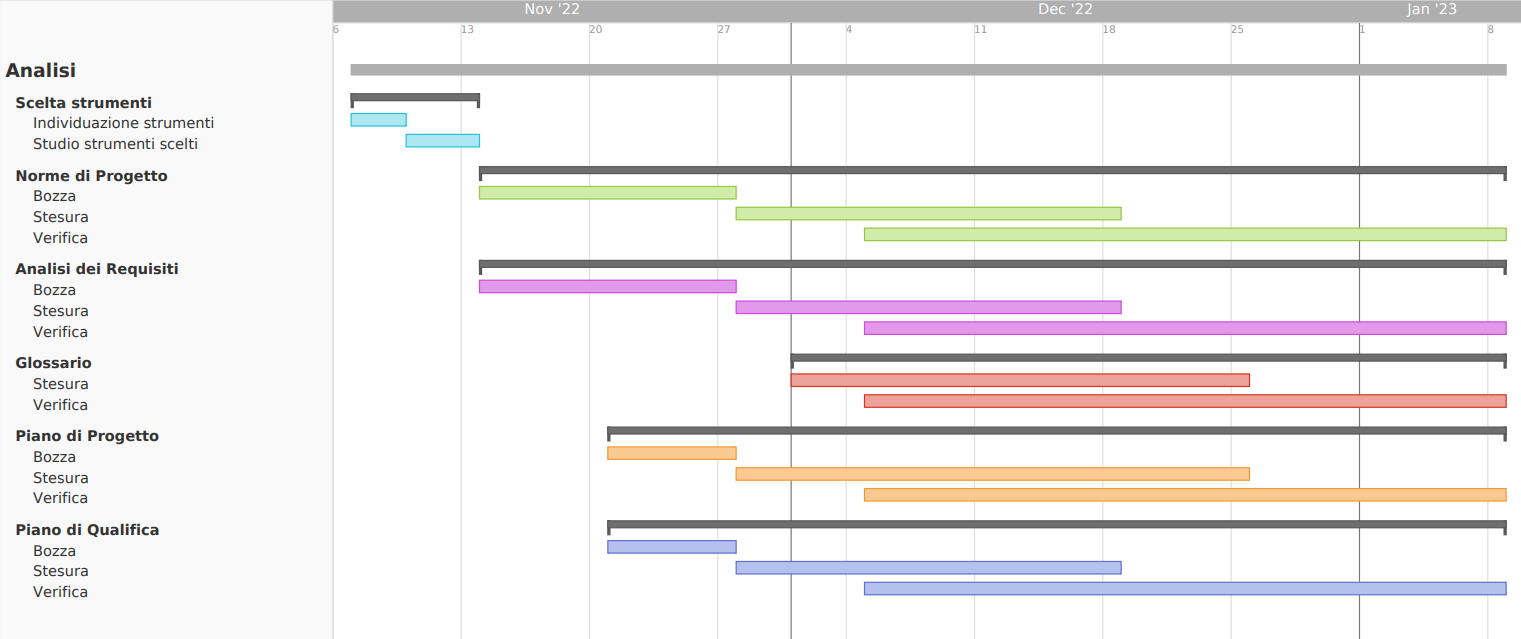
\includegraphics[width=15cm]{img/4_analisi.png}
	\caption{Esempio di diagramma di Gantt\textsubscript{G}}
\end{figure}
\paragraph {Preventivo}\mbox{}\\
In questa sezione sono contenuti i preventivi sulla distribuzione oraria del lavoro assegnato ad ogni periodo di ogni fase. Inoltre viene preventivato il costo di ogni fase e il costo totale del progetto. Ogni preventivo sarà composto da:
\begin{itemize}
	\item Due tabelle che indicano le ore e i costi necessarie per lo svolgimento del periodo;
	\item Un istogramma che illustra come sono state distribuite le ore fra i vari membri del gruppo;
	\item Un grafico a torta che mostra quanto ogni ruolo abbia inciso nel determinato periodo.
\end{itemize}
\paragraph {Consuntivo}\mbox{}\\
Iin questa sezione vengono indicati il numero di ore di lavoro impiegate e i relativi costi effettivi di ogni periodo. Questi vengono poi relazionati con i preventivi fatti nella sezione \textit{preventivo}.

\subsubsubsection{Piano\_di\_qualifica v 1.0.0}
\paragraph {Descrizione}\mbox{}\\
Questo documento stilato dai membri con il ruolo di analista e di verificatore contiene i vari obiettivi e metriche che permettono di garantire la qualità della verifica\textsubscript{G} e della validazione\textsubscript{G} dei processi e dei prodotti del progetto.
\paragraph {Struttura documento}\mbox{}\\
Questo documento è suddiviso in:
\begin{itemize}
	\item \textbf{Obiettivi e metriche di qualità di}:
	\begin{itemize}
		\item \textbf{Processo}: contiene i vari obiettivi generici e specifici e le metriche correlate ad essi che permettono la qualità di un processo;
		\item \textbf{Prodotto}: contiene i vari obiettivi e le metriche correlate ad essi che permettono la qualità di un prodotto.
	\end{itemize}
	\item \textbf{Specifiche dei test}: vengono definiti i vari test che dovranno essere eseguiti i quali sono:
	\begin{itemize}
		\item Test di unità;
		\item Test di integrazione;
		\item Test di sistema;
		\item Test di regressione;
		\item Test di collaudo.
	\end{itemize}
	\item \textbf{Resoconto delle attività di verifica}: nella quale vengono illustrati i risultati ottenuti rispetto alle metriche scelte.
	\item \textbf{Risultati dei test}: nella quale vengono inseriti i vari risultati ottenuti dai test definiti nella sezione \textit{Specifiche dei test}.
	\item \textbf{Valutazione per il miglioramento}: nella quale sono inserite le varie osservazioni e valutazioni fatte dal gruppo sia per poter migliorare l'efficacia e l'efficienza delle varie attività di verifica future, che per migliorare i risultati ottenuti nei resoconti delle verifiche.
\end{itemize} 
\paragraph {Struttura obiettivi}\mbox{}\\
Ogni obiettivo sarà contrassegnato da un codice univoco così composto:
\begin{center}
	\verb|OQ<<Tipo di obiettivo>><<ID>>|
\end{center}
Dove:
\begin{itemize}
	\item \verb|OQ| sta per obiettivo di qualità;
	\item \verb|<<Tipo di obiettivo>>| identifica se è di processo o prodotto (PC-PD);
	\item \verb|<<ID>>| è un contatore correlato al tipo di obiettivo.
\end{itemize}
\paragraph {Struttura metriche}\mbox{}\\
Ogni metrica sarà contrassegnata da un codice univoco così composto:
\begin{center}
	\verb|MQ<<Tipo di metrica>><<ID>>|
\end{center}
Dove:
\begin{itemize}
	\item \verb|MQ| sta per metrica di qualità;
	\item \verb|<<Tipo di metrica>>| identifica se è di processo o prodotto (PC-PD);
	\item \verb|<<ID>>| è un contatore correlato al tipo di metrica.
\end{itemize}

\subsubsubsection{Proof of Concept}
Un software esempio che va ad analizzare alcune sezioni critiche per lo sviluppo del progetto, osservate in seguito ad un'analisi del gruppo. Questo software permetterà al gruppo di determinare la fattibilità pratica e l'applicabilità di alcuni concetti necessari per la progettazione e codifica del prodotto finale.


\subsection{Sviluppo}
    \subsubsection{Scopo}
    L'obiettivo del processo di sviluppo è definire le attività che il gruppo deve eseguire per realizzare il prodotto finale richiesto dal proponente.
    \subsubsection{Analisi dei requisiti}
    \subsubsubsection{Scopo}
    Lo scopo di questa attività è quello di stilare tutti i requisiti\textsubscript{G} che saranno necessari per la successiva fase di progettazione e quindi per lo sviluppo di un prodotto che risponda in maniera completa ai bisogni del proponente. \\
    I requisiti individuati dovranno quindi:
    \begin{itemize}
    	\item Fornire dei riferimenti affidabili e precisi per la fase di progettazione;
    	\item Fissare le funzionalità che il prodotto finale dovrà avere; 
    	\item Aiutare a definire dei test precisi e dettagliati per agevolare le verifiche future.    	
    \end{itemize}
	\subsubsubsection{Contenuti}
    Il documento stilato dovrà quindi contenere:
    \begin{itemize}
    	\item Una descrizione generale del prodotto;
    	\item La scelta delle tecnologie da utilizzare;
    	\item L'analisi dettagliata dei casi d'uso\textsubscript{G};
    	\item I requisiti\textsubscript{G} individuati tramite:
        \begin{itemize}
            \item Documento di presentazione del capitolato;
            \item Confronti tra i membri del gruppo;
            \item Incontri con il proponente.
        \end{itemize}
    \end{itemize} 
    \subsubsubsection{Struttura dei casi d'uso\textsubscript{G}}
    Ogni caso d'uso\textsubscript{G} è identificato utilizzando la seguente convenzione di nomenclatura:
    \begin{center}
		\verb|UC<<ID_CasoBase>>.<<ID_SottoCaso>>|
    \end{center}
    Dove:
    \begin{itemize}
    	\item \verb|<<ID>>| identifica l'use case;
    	\item \verb|<<ID_SottoCaso>>| identifica eventuali sottocasi.
    \end{itemize}
	Ogni caso d'uso\textsubscript{G} è composto inoltre da:
	\begin{itemize}
		\item Descrizione: una breve descrizione dell'attività rappresentata dal caso d'uso\textsubscript{G};
		\item Attori\textsubscript{G}: entità esterne al sistema che interagiscono con esso. Ne esistono di due tipologie:
		\begin{itemize}
			\item Primario: interagisce con il sistema per raggiungere un obiettivo;
			\item Secondario: aiuta l'attore primario a raggiungere l'obiettivo.
		\end{itemize}
		\item Precondizione: descrive lo stato del sistema prima dell'attività svolta nel caso d'uso\textsubscript{G};
		\item Postcondizione: descrive lo stato del sistema dopo l'attività svolta nel caso d'uso\textsubscript{G};
		\item Scenario principale: elenco che descrive il flusso degli eventi dell'attività rappresentata dal caso d'uso\textsubscript{G};
		\item Scenari alternativi (se presenti): elenco che descrive gli eventi del caso d'uso\textsubscript{G} dopo un imprevisto che lo ha deviato dallo scenario principale;
		\item Scenari inclusi (se presenti): elenco di casi d'uso\textsubscript{G} che svolgono attività necessarie allo svolgimento dello scenario principale;
		\item Generalizzazioni (se presenti): elenco di casi d'uso\textsubscript{G} che generalizzano il caso d'uso\textsubscript{G} principale.
	\end{itemize}
    
    \subsubsubsection{Struttura dei requisiti\textsubscript{G}}
    Ogni requisito è identificato da un codice univoco così composto:
    \begin{center}
		\verb|R<<TIPOLOGIA DI REQUISITO>>-<<ID>>|
    \end{center}
    Dove:
    \begin{itemize}
        \item \verb|<<TIPOLOGIA DI REQUISITO>>| identifica una classe tra le seguenti:
        \begin{itemize}
            \item Funzionale \{F\};
            \item Qualità \{Q\};
            \item Vincolo \{V\};
            \item Prestazionale \{P\}.
        \end{itemize}
        \item \verb|<<ID>>| identifica numericamente il requisito nella classe di appartenenza.
    \end{itemize}
    Nel documento vengono raggruppati per categoria specificandone:
    \begin{itemize}
        \item Grado di obbligatorietà;
        \item Descrizione;
        \item Fonti, le quali possono essere:
        \begin{itemize}
        	\item Il capitolato d'appalto;
        	\item Verbali interni;
        	\item Verbali esterni;
        	\item I casi d'uso\textsubscript{G} identificati.
        \end{itemize}
    \end{itemize}
	
	
	\subsubsection{Progettazione}
	\subsubsubsection{Scopo e descrizione}
	Lo scopo di questa attività è quello di individuare le varie caratteristiche che comporranno il prodotto richiesto dal proponente avendo come riferimento i requisiti\textsubscript{G} e casi d'uso\textsubscript{G} definiti nel documento \textit{Analisi\_dei\_requisiti v 1.0.0}. Le varie caratteristiche verranno poi messe insieme per costruire una singola soluzione che rispetti i vari obiettivi di qualità del prodotto.
	I vari periodi in cui sarà svolta l'attività di progettazione sono:
	\begin{itemize}
		\item \textbf{Proof of concept};
		\item \textbf{Progettazione architetturale};
		\item \textbf{Progettazione di dettaglio}.
	\end{itemize}
	\subsubsubsection{Proof of concept}
	\paragraph {Scopo}\mbox{}\\
	In questa fase viene prodotto un software esempio che sarà anche la technology baseline\textsubscript{G} del prodotto finale. Questo andrà ad analizzare alcune sezioni critiche per lo sviluppo del progetto e servirà ad agevolare le successive scelte di progettazione del gruppo, aiutando a determinare la fattibilità e l'applicabilità di alcune scelte analizzate.
	\paragraph {Suddivisione periodi}\mbox{}\\
	Questa fase è divisa in due periodi:
	\begin{itemize}
		\item Periodo nel quale vengono identificati i requisiti\textsubscript{G} del \textit{Poc\textsubscript{G}} e delle 	tecnologie necessarie a svilupparlo, oltre che lo studio di queste ultime;
		\item Periodo di produzione del \textit{Poc\textsubscript{G}}.
	\end{itemize}
	\subsubsubsection{Progettazione architetturale}
	\paragraph {Scopo}\mbox{}\\
	Lo scopo di questa fase è il raffinamento della technology baseline\textsubscript{G} definita nella fase di \textit{Proof of Concept}, e discute ad alto livello l'architettura del prodotto e delle sue componenti. Le scelte che il gruppo effettua in questa fase riguarderanno la struttura complessiva del sistema e ne influenzeranno varie caratteristiche qualitative come per esempio l'efficienza, l'estensibilità e la manutenibilità.
	\subsubsubsection{Progettazione di dettaglio}
	\paragraph {Scopo}\mbox{}\\
	Lo scopo di questa fase è definire le specifiche di dettaglio dell’architettura del prodotto e di tutte le sue componenti, scomposte in unità. Queste saranno correlate a diagrammi UML\textsubscript{G} che le descriveranno e ai test di verifica\textsubscript{G} per la qualità, i quali saranno indicati nel documento \textit{Piano\_di\_qualifica v1.0.0}. Tali informazioni costituiranno la Product Baseline, la quale conterrà:
	\begin{itemize}
		\item Desing patterns utilizzati;
		\item Tecnologie utilizzate;
		\item Definizione delle classi;
		\item Tracciamento dei componenti;
		\item Diagrammi UML\textsubscript{G}:
		\begin{itemize}
			\item Diagrammi delle attività;
			\item Diagrammi delle classi.
		\end{itemize}
		\item Test di integrazione.
	\end{itemize}
	\subsubsection{Codifica}
	\subsubsubsection{Scopo e descrizione}
	La fase di \textit{Codifica} è assegnata ai membri con il ruolo di programmatore, i quali dovranno realizzare il prodotto software richiesto dal proponente utilizzando ciò che i progettisti hanno definito nella fase di \textit{Progettazione}.\\
	Per garantire un prodotto adeguato il codice dovrà essere verificato in modo che rispetti le metriche che garantiscono gli obiettivi di qualità definiti nel documento \textit{Piano\_di\_qualifica v 1.0.0}.
	\subsubsubsection{Suddivisione attività}
	Le varie attività che comporranno la fase di codifica saranno aggiunte più avanti. 

    
    
